\documentclass[12pt,landscape]{article}
\usepackage[left=0.1in, right=0.1in, top=0.6in,bottom=0.1in]{geometry}
\usepackage{enumitem}
\usepackage{amsmath}
\usepackage{tikz}
\usepackage{ulem}
\usetikzlibrary{shapes.geometric, arrows.meta, positioning, calc}

% --- Tikz set for diagram
\tikzset{
    box/.style={rectangle, draw, minimum width=1.8cm, minimum height=1cm, align=left, font=\small},
    doublebox/.style={rectangle, draw, double, double distance=1.5pt, minimum width=2.5cm, minimum height=1cm, align=left, font=\small},
    decision/.style={diamond, draw, minimum width=1cm, minimum height=1cm, align=center, aspect=2, font=\small},
    doubledecision/.style={diamond, double, draw, minimum width=1cm, minimum height=1cm, align=center, aspect=2, font=\small},
    attribute/.style={rectangle, draw, minimum width=1.5cm, minimum height=0.6cm, align=center, font=\small},
    arrow/.style={-Stealth, thick},
    doublearrow/.style={-Stealth, thick, double, double distance=1.5pt},
    dashedline/.style={thick, dashed},
    line/.style={thick},
    doubleline/.style={thick, double, double distance=1.5pt}
}

\begin{document}

\begin{center}
{\huge\bfseries Schema Diagram for University Database}

\vspace{0.5cm}
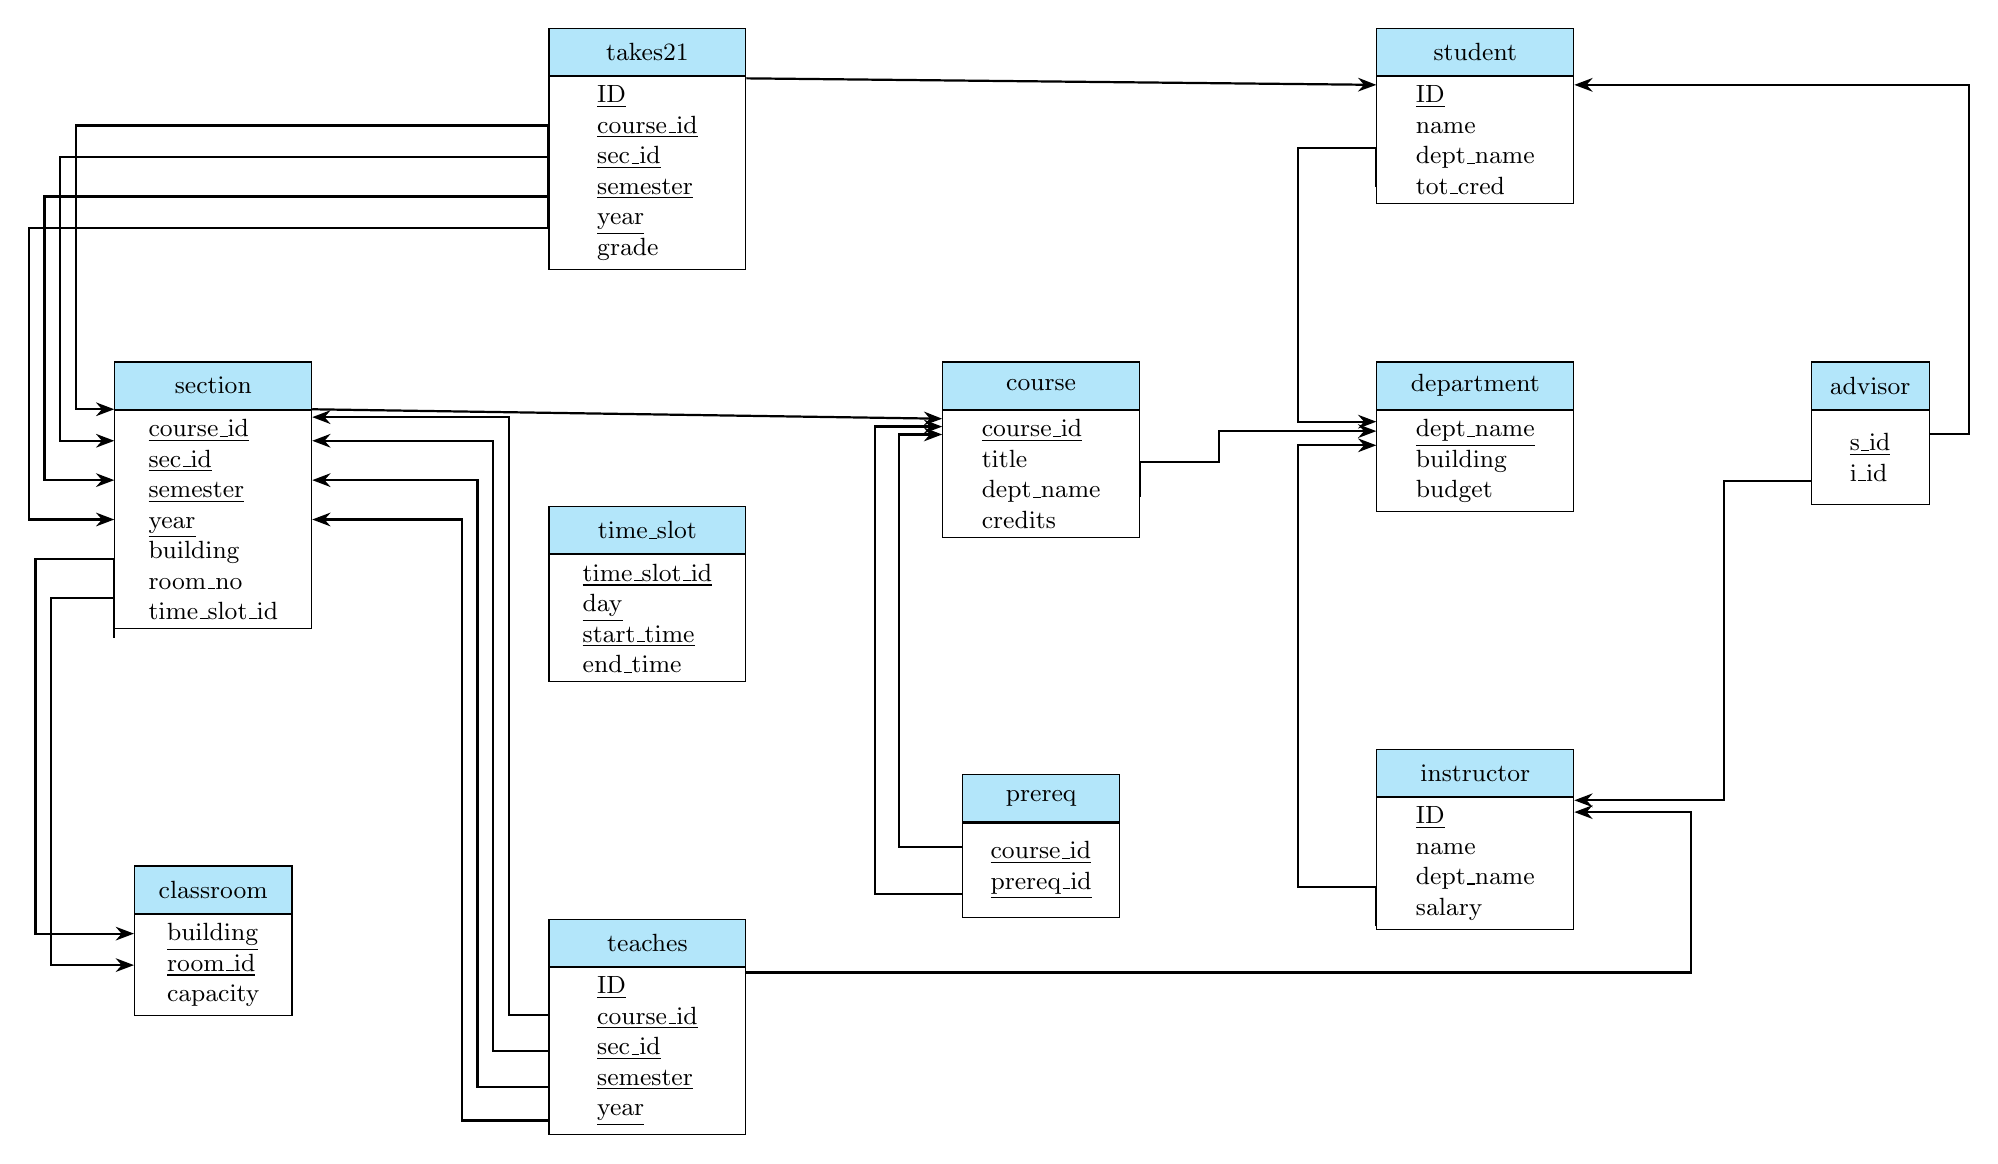
\begin{tikzpicture}[node distance=2cm]
    % Takes table
    \node[box, fill=cyan!30, minimum height=0.6cm, minimum width=2.5cm] (takes_header) {takes21};
    \node[box, fill=white, below=0cm of takes_header.south, anchor=north, minimum height=1.2cm, minimum width=2.5cm] (takes_body) {\underline{ID}\\\underline{course\_id}\\\underline{sec\_id}\\\underline{semester}\\\underline{year}\\grade};
    
    % time_slot table
    \node[box, fill=cyan!30, minimum height=0.6cm, minimum width=2.5cm, below=3cm of takes_body] (time_slot_header) {time\_slot};
    \node[box, fill=white, below=0cm of time_slot_header.south, anchor=north, minimum height=1.5cm, minimum width=2.5cm] (time_slot_body) {\underline{time\_slot\_id}\\\underline{day}\\\underline{start\_time}\\end\_time};

    % teaches table
    \node[box, fill=cyan!30, minimum height=0.6cm, minimum width=2.5cm, below=3cm of time_slot_body] (teaches_header) {teaches};
    \node[box, fill=white, below=0cm of teaches_header.south, anchor=north, minimum height=1.2cm, minimum width=2.5cm] (teaches_body) {\underline{ID}\\\underline{course\_id}\\\underline{sec\_id}\\\underline{semester}\\\underline{year}};
    
    % student table
    \node[box, fill=cyan!30, minimum height=0.6cm, minimum width=2.5cm, right=8cm of takes_header] (student_header) {student};
    \node[box, fill=white, below=0cm of student_header.south, anchor=north, minimum height=1.2cm, minimum width=2.5cm] (student_body) {\underline{ID}\\name\\dept\_name\\tot\_cred};

    % department table
    \node[box, fill=cyan!30, minimum height=0.6cm, minimum width=2.5cm, below=2cm of student_body] (department_header) {department};
    \node[box, fill=white, below=0cm of department_header.south, anchor=north, minimum height=1.2cm, minimum width=2.5cm] (department_body) {\underline{dept\_name}\\building\\budget};

    % instructor table
    \node[box, fill=cyan!30, minimum height=0.6cm, minimum width=2.5cm, below=3cm of department_body] (instructor_header) {instructor};
    \node[box, fill=white, below=0cm of instructor_header.south, anchor=north, minimum height=1.2cm, minimum width=2.5cm] (instructor_body) {\underline{ID}\\name\\dept\_name\\salary};

    % course table
    \node[box, fill=cyan!30, minimum height=0.6cm, minimum width=2.5cm, left=3cm of department_header] (course_header) {course};
    \node[box, fill=white, below=0cm of course_header.south, anchor=north, minimum height=1.2cm, minimum width=2.5cm] (course_body) {\underline{course\_id}\\title\\dept\_name\\credits};

    % advisor table
    \node[box, fill=cyan!30, minimum height=0.6cm, minimum width=1.5cm, right=3cm of department_header] (advisor_header) {advisor};
    \node[box, fill=white, below=0cm of advisor_header.south, anchor=north, minimum height=1.2cm, minimum width=1.5cm] (advisor_body) {\underline{s\_id}\\i\_id};

    % prereq table
    \node[box, fill=cyan!30, minimum height=0.6cm, minimum width=2.0cm, below=3cm of course_body] (prereq_header) {prereq};
    \node[box, fill=white, below=0cm of prereq_header.south, anchor=north, minimum height=1.2cm, minimum width=2.0cm] (prereq_body) {\underline{course\_id}\\\underline{prereq\_id}};

    % section table
    \node[box, fill=cyan!30, minimum height=0.6cm, minimum width=2.5cm, left=8cm of course_header] (section_header) {section};
    \node[box, fill=white, below=0cm of section_header.south, anchor=north, minimum height=1.2cm, minimum width=2.5cm] (section_body) {\underline{course\_id}\\\underline{sec\_id}\\\underline{semester}\\\underline{year}\\building\\room\_no\\time\_slot\_id};

    % classroom table
    \node[box, fill=cyan!30, minimum height=0.6cm, minimum width=2.0cm, below=3cm of section_body] (classroom_header) {classroom};
    \node[box, fill=white, below=0cm of classroom_header.south, anchor=north, minimum height=1.2cm, minimum width=2.0cm] (classroom_body) {\underline{building}\\\underline{room\_id}\\capacity};


    % Lines and arrows
    \draw[arrow] ([yshift=1.2cm]takes_body.east) -- ([yshift=0.7cm]student_body.west);
    
    % section to takes (4 bundled lines: course_id, sec_id, semester, year)
    \draw[arrow] (takes_body.west) |- ++(-6,0.6) |- ([yshift=1.4cm]section_body.west);
    \draw[arrow] (takes_body.west) |- ++(-6.4,-0.3)  |-  ([yshift=0.5cm]section_body.west);
    \draw[arrow] (takes_body.west) |- ++(-6.2,0.2)  |-  ([yshift=1cm]section_body.west);
    \draw[arrow] (takes_body.west) |- ++(-6.6,-0.7) |-  (section_body.west);
    
    % section to course (single arrow from course_id)
    \draw[arrow] ([yshift=1.4cm]section_body.east) -- ([yshift=0.7cm]course_body.west);
    
    % section to classroom (2 lines: building, room_no)
    \draw[arrow] ([yshift=-1cm]section_body.west) |- ++(-1,0.5) |- ([yshift=0.4cm]classroom_body.west);
    \draw[arrow] ([yshift=-1.5cm]section_body.west) |- ++(-0.8,0.5) |- (classroom_body.west);
    
    % course to department (single arrow from dept_name)
    \draw[arrow] ([yshift=-0.3cm]course_body.east) |- ++(1,0.45) |- ([yshift=0.38cm]department_body.west);
    
    % student to department (single arrow from dept_name)
    \draw[arrow] ([yshift=-0.6cm]student_body.west) |- ++(-1,0.5) |- ([yshift=0.5cm]department_body.west);
    
    % instructor to department (single arrow from dept_name)
    \draw[arrow] ([yshift=-0.8cm]instructor_body.west) |- ++(-1,0.5) |- ([yshift=0.2cm]department_body.west);

    % teaches to instructor(single arrow from teaches)
    \draw[arrow] ([yshift=1cm]teaches_body.east) -- ++(12,0) |- ([yshift=0.65cm]instructor_body.east);
     
    % teaches to section (4 bundled lines going up: course_id, sec_id, semester, year)
    \draw[arrow] (teaches_body.160) -- ++(-0.5,0) |- ([yshift=1.3cm]section_body.east);
    \draw[arrow] (teaches_body.180) -- ++(-0.7,0) |- ([yshift=1cm]section_body.east);
    \draw[arrow] (teaches_body.200) -- ++(-0.9,0) |- ([yshift=0.5cm]section_body.east);
    \draw[arrow] (teaches_body.215) -- ++(-1.1,0) |- (section_body.east);
    
    % advisor to student (arrow from s_id going up to student)
    \draw[arrow] ([yshift=0.3cm]advisor_body.east) -- ++(0.5,0) |- ([yshift=0.7cm]student_body.east);
    
    % advisor to instructor (arrow from i_id going down to instructor)
    \draw[arrow] ([yshift=-0.3cm]advisor_body.west) -- ++(-1.1,0) |- ([yshift=0.8cm]instructor_body.east);
    
    % prereq to course (2 arrows: course_id and prereq_id)
    \draw[arrow] ([yshift=-0.3cm]prereq_body.west) -- ++(-1.1,0) |- ([yshift=0.6cm]course_body.west);
    \draw[arrow] ([yshift=0.3cm]prereq_body.west) -- ++(-0.8,0) |- ([yshift=0.5cm]course_body.west);

    
\end{tikzpicture}
\end{center}
\end{document}